\begin{problem}{지구이웨를 둘러보다}
	{standard input}{standard output}
	{4 seconds}{128 megabytes}{}
	
	지구이웨에는 $n$개의 마을이 있다. 몇몇 두 마을은 양방향 도로로 연결되어있다. 도로들은 양 끝점에서 만나고, 교차하지 않는다. 터널이나 고가도로가 있기에 가능한 일이다.
	
	이제 곧 유명한 자전거 경주인 ``지구이웨를 둘러보다"가 열린다. 경주는 지구이웨이 있는 도로들을 사용하고, 시작도시와 끝 도시가 같으며, 모든 도로를 최대 한번만 지난다는 점이 알려져 있다.
	
	범수는 유명한 에밀리아 팬클럽의 회장이다. 범수와 그의 팬클럽 동료들은 자전거 경주를 싫어한다. 그들은 자전거 경주의 도로가 자기가 살고 있는 마을을 통과하지 못하게 몇몇 도로들을 막고싶어 한다. 범수는 클럽의 회원들이 어떤 마을에 사는지 알고 있고, 그들이 살고 있는 마을을 경주로 사용하지 못하게 하는 최소한의 도로 수를 알고 싶어 한다. 자세히는, 모든 가능한 경주가 어떤 마을도 통과하지 않게 하고 싶다. 범수를 위해 그런 도로들을 찾아주자.
	

	\InputFile
	
	입력에 첫째 줄에는 공백 하나로 구분된 세 개의 정수 $n$, $m$, $k$가 주어진다. ($1 \le n \le 1,000,000$, $0 \le m \le 2,000,000$, $1\le k \le n$) 이 수는 각각 마을의 수, 도로의 수, 팬클럽 멤버들이 살고 있는 도시의 수를 나타낸다. 마을은 1부터 $n$까지 번호가 붙어있고 팬클럽 멤버들은 1번 마을부터 $k$번 마을까지 살 고 있다. 다음 $m$개의 줄에는 공백 하나로 구분된 두 개의 수 $a_i$ 와 $b_i$($1 \le a_i < b_i \le n$)가 주어진다. 이는 $a_i$와 $b_i$ 사이에 양방향 도로가 존재함을 의미한다. 지구이웨의 두 마을은 최대 한 개의 도로로만 연결되어있다.

	\OutputFile
	
	프로그램은 범수의 팬클럽 회원들이 살고 있는 마을을 경주로 사용하지 못하게 하기 위해 막야아 하는 도로들의 집합 중 크기가 최소인 것을 찾아야 한다.
	
	첫째 줄에는 그 도로들의 크기를 출력한다. 다음에 한 줄에 하나 씩 막아야 하는 도로들을 출력한다. 도로는 양 끝점을 공백 하나로 구분하여 출력해야 하고, 번호가 작은 도시가 큰 도시보다 먼저 와야 한다.
	
	답이 여러개인 경우 아무거나 출력하여도 좋다.
	
	\SubtaskWithCost{1}{40}
	\begin{itemize}
		\item $n \le 1,000$
		\item $m \le 5,000$
	\end{itemize}
	
	\SubtaskWithCost{2}{60}
	
	추가 제한조건이 없다.
	
	\Examples
		
	\begin{example}
	\exmp{
11 13 5
1 2
1 3
1 5
3 5
2 8
4 11
7 11
6 10
6 9
2 3
8 9
5 9
9 10
	}{%
3
2 3
5 9
3 5
	}%
	\end{example}
	
	\Note
	
	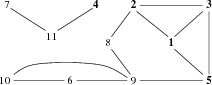
\includegraphics[]{tou.png}
	
\end{problem}

